%  ALU_Design.tex
%  Document created by seblovett on seblovett-Ubuntu
%  Date created: Thu 17 Apr 2014 15:00:33 BST
%  <+Last Edited: Mon 05 May 2014 11:39:09 BST by seblovett on seblovett-Ubuntu +>


\section{Arithmetic Logic Unit}\label{sect:design:alu}
\todo[color=cyan, inline]{Design of whole module - ongoing}
\todo[color=cyan, inline]{Use of hierarchy - implied mention, todo}
\todo[color=cyan, inline]{Design of slice - initial text done}
\todo[color=cyan, inline]{Design of decoder - initial text done}
\todo[color=cyan, inline]{Design of block - initial test done}
\todo[color=cyan, inline]{Layout in silicon}

The arithmetic logic unit (ALU) is the central unit for performing calculations within the datapath. 
Most instructions use the ALU as part of their operation and as such this module needs to interpret every instruction and perform the necessary function. 
The range of functions needed fall into one of four types: arithmetic, logic, shifting and load lower. 
With the last type being a special case for the LLI instruction. 
Arithmetic operations are centralized around a full adder with additional gates for subtraction, setting the first input to zero and flag calculations. 
The logic unit consists of one gate corresponding to each of the full set of logic instructions supported. 
While shifts are performed using a barrel shifter to support up to 15-bits in one clock cycle. 
Finally, the LLI module concatenates the upper byte of the destination register with the provided 8-bit immediate value. 
The breakdown of the ALU is illustrated in Figure~\ref{fig:abstractALU}, with the output of each section connected to an internal bus through a number of tri-state gates. 


\begin{figure}[h]
	\centering
	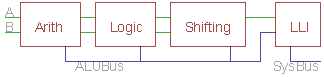
\includegraphics[width=3in]{Figures/AbstractALU.png}
	\caption{ALU Separated into Sub-modules}
	\label{fig:abstractALU}
\end{figure}

This design then needed to be bit-sliced to simplify the datapath and promote hierarchical construction. 
It was decided to add an additional input to the module for the 4-bit immediate value required to define the shifting amount. 
Otherwise the lowest four bits of the ALU will each need a different routing to each segment, reducing how much of each slice could be identically duplicated. 
\todo[inline,color=green]{HSL - @MW tenses change in this. Should be past - ``it was designed in bit slices\dots''}

Initial design of the ALU module was based upon the planned datapath layout and the input/output connections it showed, as seen in Figure~\ref{fig:BasicALUSym}. 
From this it was seen that there may be some difficulty with interpreting the opcodes provided. 
Since each slice would have to individually interpret the opcode, using much more space than is necessary due to replicated hardware. 
Observations showed that different groups of instructions would perform the same operation within the ALU. 
As such, it was decided to use a separate decoder to interpret the opcodes and send control lines to the ALU for the specific functions to be performed. 
\todo[inline,color=green]{HSL - @MW - I don't think this aids to any understanding. 
The final point is key, but could be condensed down into one/two lines and joined with the above. 
Maybe ``To reduce the bitslice size, all decoding logic was implemented in an extra decoding module.''}

\begin{figure}[h]
	\centering
	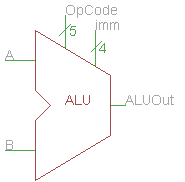
\includegraphics[width=1.5in]{Figures/ALUTopLevel.png}
	\caption{Initial Top-level View of ALU Module}
	\label{fig:BasicALUSym}
\end{figure}

\subsection{ALU Slice}
%The most beneficial bit slice would be one that performs all the functions required for one bit and as such can be replicated to produce a 16-bit datapath. 
%As such design focussed upon this idea, with considerations towards the overall size of the ALU once built. 
The arithmetic section was simple to bitslice since the full adder and input selection gates would be duplicated for each bit anyway. 
While the flags required only one OR gate for the Z flag and the sum, carry in and carry out signals to be available at the top of the slice. 
Since a decoder is positioned at the top, additional gates needed for flag calculation can be implemented once within the decoder. 
This is shown in Figure~\ref{fig:ArithSlice}. 
Bit slicing the logic section was just one of each logic gate followed by a tri-state buffer in the slice, shown in Figure~\ref{fig:LogicSlice}. 


\begin{figure}[h]
	\centering
	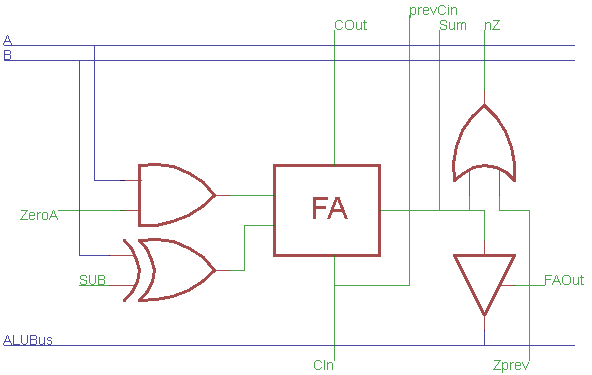
\includegraphics[width=3in]{Figures/ArithSlice.png}
	\caption{Bitsliced Ciruit Diagram for Arithmetic Section of ALU}
	\label{fig:ArithSlice}
\end{figure}

\begin{figure}[h]
	\centering
	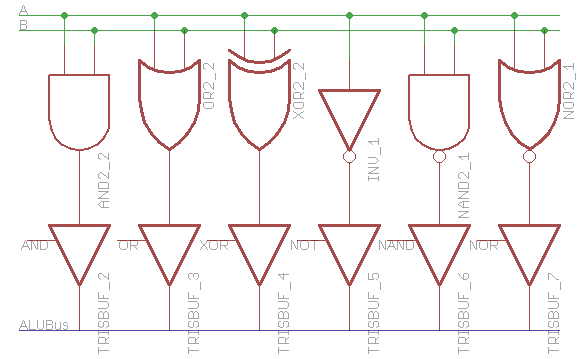
\includegraphics[width=3in]{Figures/LogicSlice.png}
	\caption{Bitsliced Ciruit Diagram for Logic Section of ALU}
	\label{fig:LogicSlice}
\end{figure}

Implementing shifting capabilities into individual bits required few logic gates since it is a wire-dominated circuit, but each wire needed to be lined up correctly between slices. 
This results from this slice section having more dependency on the neighbouring slices than both arithmetic and logic functions. 
The left and right shifting have been implemented using separate hardware. 
To support arithmetic shifting, the shifted value into a right shift can be either a zero and the current operand's sign.
Implementation of this section is shown in Figure~\ref{fig:ShiftSlice}. 

\begin{figure}[h]
	\centering
	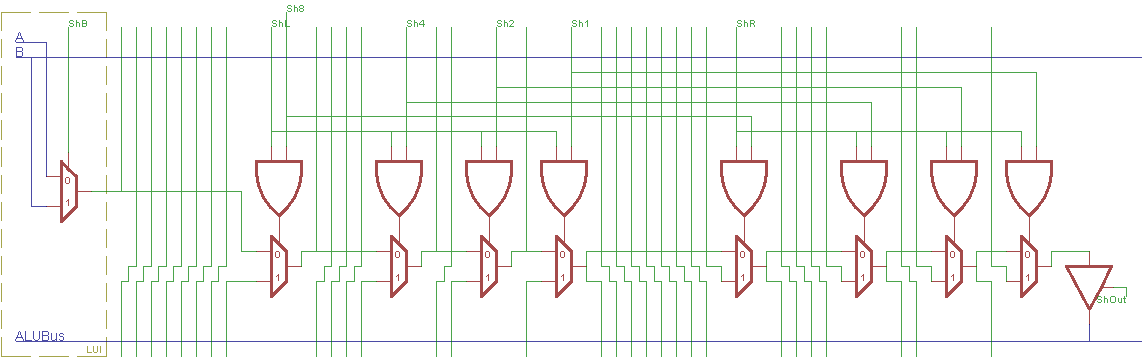
\includegraphics[width=\textwidth]{Figures/ShiftSlice.png}
	\caption{Bitsliced Ciruit Diagram for Shift Section of ALU}
	\label{fig:ShiftSlice}
\end{figure}

Every instruction can be carried out using one of the previous sections, with the exception of LUI and LLI. Loading an upper immediate value involves concatenating the 8-bit value with 8 zero bits. 
This is equivalent to shifting the second operand by 8-bits, as such it can be implemented with an additional multiplexor before the shifting section to select between each input operand. 
This is shown in Figure~\ref{fig:ShiftSlice} as a precurser to standard shifting operation. 
Loading a lower immediate involves concatenating the existing high byte of the destination register with the value in the instruction. 
However there is no way of separating this into 16 identical slices. 
As such two versions of the slice were designed, one which passes through the upper byte with no change, and one which selects between the lower byte of the input register value and the immediate value. 
These form modules which are separate to the main slice, with the lower slice shown in  Figure~\ref{fig:LLISlice}, therefore LLI functionality is not part of the main ALU. 

\begin{figure}[h]
	\centering
	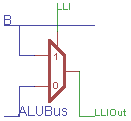
\includegraphics[width=1.5in]{Figures/LLILSlice.png}
	\caption{Bitsliced Ciruit Diagram for LLI Modules}
	\label{fig:LLISlice}
\end{figure}

\subsection{ALU Decoder}
The purpose of a decoder module is to convert any given opcode into a number of signals to control the path of data within the ALU. As such it is composed of multiple circuits of purely combinational logic. Table~\ref{tab:contrOuts} shows the necessary control signals for each mnemonic.


\begin{table}[h]
	\centering
	\footnotesize
	\makebox[\linewidth]{
	\begin{tabular}{|r|l|l|c|r|l|l|}
		\multicolumn{2}{c}{Instruction} & \multicolumn{1}{c}{Decoder Outputs} & \multicolumn{1}{c}{\hspace{0.5cm}} & \multicolumn{2}{c}{Instruction} & \multicolumn{1}{c}{Decoder Outputs} \\
		\cline{1-3} \cline{5-7} 
		LDW   & 00000 & FAOut &  & NOP   & 11000 & ShOut \\
		POP   & 00001 & FAOut &  & 'F'   & 11001 & ShOut \\
		ADDIB & 00011 & FAOut &  & NEG   & 11010 & FAOut, SUB, ZeroA \\
		ADD   & 00010 & FAOut &  & 'D'   & 11110 & FAOut \\
		ADDI  & 00110 & FAOut &  & LSL   & 11111 & ShOut, ShL, \{Sh8-1\} \\
		CMP   & 00111 & FAOut, SUB &  & LSR   & 11101 & ShOut, ShR, \{Sh8-1\} \\
		ADCI  & 00101 & FAOut, {\it UseC} &  & ASR   & 11100 & ShOut, ShR, {\it ShSign}, \{Sh8-1\} \\
		ADC   & 00100 & FAOut, {\it UseC} &  & AND   & 10000 & AND \\
		STW   & 01000 & FAOut &  & OR    & 10001 & OR \\
		PUSH  & 01001 & FAOut, SUB &  & XOR   & 10011 & XOR \\
		SUBIB & 01011 & FAOut, SUB &  & NOT   & 10010 & NOT \\
		SUB   & 01010 & FAOut, SUB &  & NAND  & 10110 & NAND \\
		SUBI  & 01110 & FAOut, SUB &  & NOR   & 10111 & NOR \\
		CMPI  & 01111 & FAOut, SUB &  & LLI   & 10101 & ShOut, LLI \\
		SUCI  & 01101 & FAOut, SUB, {\it UseC} &  & LUI   & 10100 & ShOut, ShL, ShB, Sh8 \\
		SUC   & 01100 & FAOut, SUB, {\it UseC} &  & & 11011 & ShOut \\
		\cline{1-3} \cline{5-7}
	\end{tabular}
	}
	\caption{Control outputs for each available instruction mnemonic}
	\label{tab:contrOuts}
\end{table}
\todo[inline]{check what 11011 does}

The signal FAOut enables the tri-state buffer of the arithmetic section. 
SUB inverts the second input and flags for a subtraction operation and ZeroA sets the first input to zero. 
The logic tri-states are controlled by the signals AND, OR, XOR, NOT, NAND and NOR for the relevant logic operations. 
The signal ShOut enables the tri-state for the shifting section and if used with nothing else active has the effect of no operation being performed on data. 
ShL and ShR switch between left and right shifting while ShB switches between using the first (A) or second (B) input to shift. 
Signals Sh8, Sh4, Sh2 and Sh1 enable each section of the barrel shifter and during normal shifting operations are dependent upon the 4-bit immediate input to decoder. 
Sh8 is set during a LUI instruction since it will always shift by 8 bits. 
Signal LLI activates the LLI module after no operation is performed within main ALU. 
While UseC and ShInBit are internal signals indicating use of the carry flag from previous instruction and the bit to shift in respectively. 
The one unused opcode is set to perform no operation on data to prevent unpredictable behaviour. 
\todo[inline,color=green]{HSL - @MW can you condense this? It's a bit dry. Maybe say ``Signals FAOut, AND, OR \dots are used to enable relevant tristate buffers to output the result. It uses one hot coding to prevent contention.'' and similar. }

\begin{align}
	\text{FAOut} &= \bar{A} + BD\bar{E} \label{eq:DecBasicS}\\
	\text{SUB} &= \bar{A}BC + \bar{A}B\bar{C}E + B\bar{C}D\bar{E} + \bar{A}CDE \\
	\text{ShL} &= \\
	\text{Sh8} &= (ABCE + ABC\bar{D})imm[3] + A\bar{B}C\bar{D}\bar{E} \label{eq:DecBasicF} \\
	\text{Sh4} &= (ABCE + ABC\bar{D})imm[2] \\
	\text{Sh2} &= (ABCE + ABC\bar{D})imm[1] \\
	\text{Sh1} &= (ABCE + ABC\bar{D})imm[0] \\
	\text{ShOut} &= AC\bar{D} + ABCE + AB\bar{C}\bar{D} \\
	\text{UseC} &= \bar{A}C\bar{D} \\
	\text{ShR} &= ABC\bar{D}
\end{align}
\todo[inline]{ShL}

By using the opcodes and k-map groupings defined in Tables~\ref{tab:OpKmapA}~and~\ref{tab:OpKmapB}, logic equations have be formed as shown in Equations~\ref{eq:DecBasicS}~to~\ref{eq:DecBasicF}. 
Where the letters A-E correspond to bits 4-0 of the opcode. 
Refining these equations for implementation considered the set of logic gates available within the library, as well as the number of gates needed. 
The possible gates essential to the decoder were: and2, or2, nand2, nand3, nand4, nor2 and nor3. Where each number corresponds to the amount of logic inputs. 
Since the negated output gates had more possible inputs, as well as being physically smaller, they were more favourable to use. 
Some potential options for the logic equation for the ``SUB'' signal are shown in Equations~\ref{eq:DecSUB1}~and~\ref{eq:DecSUB2}. 
The first one, taken from the k-map, requires 1 and3, 4 and4's, 1 or4 and 3 inverters. 
To simplify design, inverters are not considered towards optimum design as both inverted and non-inverted inputs will be made available globally. 
This equation is not possible to implement due to AND gates with more than 2 inputs. 
Equation~\ref{eq:DecSUB2} requires 2 and2's, 3 and3's, and 3 or2's which again cannot be implemented. 
However if inverted using DeMorgan's law to produce Equation~\ref{eq:DecSUB3} it is possible, and uses 8 smaller gates. 
Since no further improvements could be made, this final equation is used and implemented in Figure~\ref{fig:DecMultiCirs}. 
A similar approach is taken for the remaining signals listed in Equations~\ref{eq:DecBasicS}~to~\ref{eq:DecBasicF}, with the final circuit diagrams also shown in Figure~\ref{fig:DecMultiCirs}. 
\todo[inline,color=green]{HSL - @MW I don't think this aids any understanding. Maybe just give the final equations implemented with reason of optimising to reduce number of gates.}

\newcommand{\overbar}[1]{\mkern 1.5mu\overline{\mkern-1.5mu#1\mkern-1.5mu}\mkern 1.5mu}
\begin{align}
	\text{SUB} &= \bar{A}BC + \bar{A}B\bar{C}E + B\bar{C}D\bar{E} + \bar{A}CDE \label{eq:DecSUB1}\\
	&= \bar{A}B(C + \bar{C}E) + D(B\bar{C}\bar{E} + \bar{A}CE) \label{eq:DecSUB2}\\
	%&= \bar{A + \bar{B} + \bar{(p)}} \label{eq:DecSUB3} %(\bar{C}\bar{(c + \bar{E})})
	&= \overbar{\overbar{(\bar{A}B\overbar{(\bar{C}\overbar{(\bar{C}E)})})}\overbar{(D\overbar{(\overbar{(B\bar{C}\bar{E})}\overbar{(\bar{A}CE)})})}} \label{eq:DecSUB3}
\end{align}
\todo[inline]{check against implimented}
\todo[inline]{are all final equations needed as above?}

\begin{figure}[h]
	\centering
	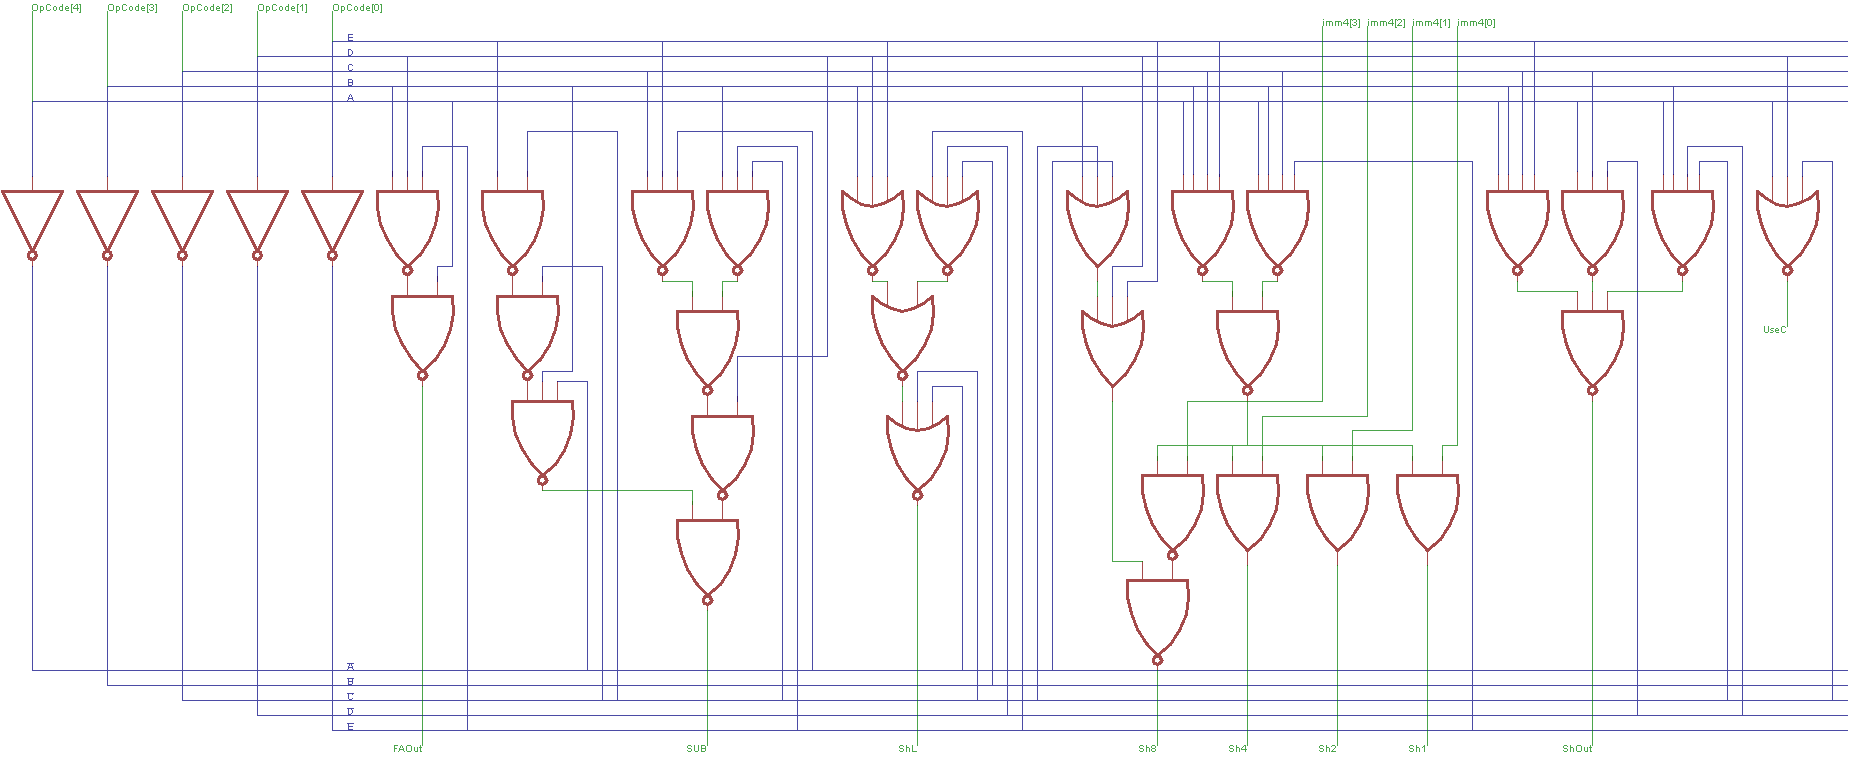
\includegraphics[width=\textwidth]{Figures/ALUDecoderMore1.png}
	\caption{Circuit Diagrams For Signals Active For More Than One Opcode}
	\label{fig:DecMultiCirs}
\end{figure}

For the control signals which respond to only one opcode, a gate array was used, as shown in Figure~\ref{fig:GateArray}. 
Since additional logic for flag calculations are implemented in the decoder, the circuit diagram for this portion is also shown in Figure~\ref{fig:GateArray}. 
\todo[inline,color=green]{HSL - @MW this makes no sense to me}

\begin{figure}[h]
	\missingfigure{Circuit Diagrams For Gate Array and Flag Overhead Logic}
	\caption{Circuit Diagrams For Gate Array and Flag Overhead Logic}
	\label{fig:GateArray}
\end{figure}

\subsection{ALU Block}
The final hierarchical view of the assembled ALU made up of each part mentioned previously is shown in Figure~\ref{fig:ALUAssembled}. 
ALU slice is duplicated to make up the 16 bits in parallel, LLI high is added to the top byte and LLI low is added to the bottom half. 
The decoder is added above, with additional wiring to connect together right shifting inputs. 
While the left shifting inputs at the bottom are tied low. 
The output to the ALU is available as a direct connection to elsewhere in the datapath, but it is also stored in a register for later transfer onto the system bus. 
This register forms a part of a separate module to the ALU. 

\begin{figure}[h]
	\missingfigure{Modular Diagram of Assembled ALU}
	\caption{Modular Diagram of Assembled ALU}
	\label{fig:ALUAssembled}
\end{figure}
